% Adapted from Jennifer Pan, August 2011

\documentclass[10pt,letter]{article}
\usepackage{amsmath}
\usepackage{amssymb}
\usepackage{graphicx}
\usepackage{setspace}

\onehalfspacing % text become 1.5 spaced

\usepackage{fullpage}
\usepackage{tikz}

\newcommand{\hongzi}[1]{{{\color{red}(HM: #1)}}}
	
\begin{document}


\title{6.854 Problem Set 1}

\author{Hongzi Mao}

\date{September 16, 2016}
 
\maketitle 

\section*{Problem 1}
\paragraph{(a)} We transform this problem to a problem similar to Planer Point Location and use persistent red-black tree to solve it, as in Figure \ref{fig:1-1}. 

\subparagraph{algorithm}In the preparation step, we separate the interval `in another dimension' and slab them based on their boundaries. Then the problem visually intuitively becomes, finding the `narrowest' slab that contained the point, and return all the interval that the slab cuts through.

We construct a persistent red-black tree, by making real-line the time dimension. Every time the left boundary of an interval is hit, the slab location is inserted into the tree (in that version of time); likewise when right boundary is hit, the slab is deleted from the tree. 

In the search step, we search the nearest slabs for the point via binary search in time, then output all nodes in the tree (all intervals in that version of the tree).
\subparagraph{analysis} The insert and delete operation in persistent red-black tree takes $O(1)$ space (optimized red-black tree, the current version remembers $O(log\:n)$ red-black bit, only the connection is persisted), so the space takes $O(n)$. Insert and delete takes $O(log\:n)$ time, so the total construction time is $O(n\:log\:n)$.

The finding `nearest slab' step takes $O(log\:n)$ time and output all containing interval in that version of tree takes $O(k)$ time, so in total it takes $(k + log\:n)$ time.
\begin{figure}
	\centering
	\includegraphics[width=0.4\textwidth]{1-1.jpg}
	\caption{Transform interval searching problem into planer-point-location-like problem.} \label{fig:1-1}
\end{figure}
\paragraph{(b)} If the interval is integer based, instead of a persistent tree, we can do a persistent linked list. Every time we do an insert, it stores the pointer (because it is integer we can map all integers in that range to a pre-allocated array to store the linked list ) to the linked list as well, in order for $O(1)$ time access. The delete operation is also $O(1)$ time. Therefore the total construction time and space will be $O(n)$. Finding the nearest slab takes $O(1)$ time (in the construction step, while adding interval boundary we can mark each entry the nearest slab), and outputting the interval in that version takes $O(k)$ time.

\pagebreak 

\section*{Problem 2}

\paragraph{(a)} The intuition is to persist each node with pointers to its $2^k$ ancestor node, where $k = \{1, 2, ..., \lfloor log_2(n)\rfloor\}$, in order to do exponential search. Then query would search the least ancestor node for the pair by walking exponentially up then decrease. 

\subparagraph{algorithm}
In the preprocessing, while traversing the tree, maintain an array storing the nodes to the root, such that each node visited can map its parent, parent of parent, $2^2$'s ancestor, $2^3$'s ancestor ... to each node and store. Maintain a balanced BST for the entry of each node. The preprocessing time and space will be $O(n\:log\:n)$.

In the $query(u,v)$ step, without loss of generality, assume $depth(u) \leq depth(v)$. We first jump the pointer of $u$ to an ancestor $u'$ such taht $depth(u') = depth(v)$. This is done by first setting $k = \lfloor log_2(n)\rfloor$. Then if $2^k$ ancestor overshoots, it reduces $k$ by one; otherwise it jumps to the ancestor and uses \emph{the same} $k$ and repeat; until hits the same depth as $v$.

Starting here, we can use the same approach as above. Notice that the common ancestor will have the same `distance' to both $p$ and $q$, so we need to jump them together until they meet at the lowest common node. Again we set $k = \lfloor log_2(n)\rfloor$. If $2^k$ ancestors of both of them are the same, it reduces $t$ by one; otherwise it jumps to the ancestor and uses \emph{the same} $k$ and repeat; until $k=0$. It first finds an ancestor of $u$ and $v$ then walk back the find the lowest common ancestor.

\subparagraph{analysis}
The query time in the first step of finding $u$ and $v$ in persistent tree is $O(log\:n)$. In the second step of making $u'$ and $v$ in the same level takes $O(log\:n)$ because of exponential search. In the second step is also $O(log\: n)$ because there is at most $O(log\: n)$ to jump and $O(log\: n)$ steps to reduce $k$ by 1. Therefore total query time is $O(log\:n)$.

\paragraph{(b)} Because the number of node is given in a priori we can map them into an integer array. The storing of the root of the node in a particular version can then be in a persistent linked list, which therefore gives $O(n)$ preprocessing time.

\pagebreak

\section*{Problem 3}
\paragraph{(a)} 
Denote the $n$ nodes by $a_1, a_2, ..., a_n$, then the linked list shaped tree is

\begin{tikzpicture}[scale=0.5]
\node{$a_n$}
child{
	node{$a_{n-1}$} 
	child{
		node {...}
		child{
			node{$a_2$}
			child{
				node{$a_1$}
			}
			child[missing]
		}
		child[missing]
		} 
	child[missing] 
	}
child[missing];
\end{tikzpicture}.
After the \emph{single} rotation, the resulting tree is \begin{tikzpicture}[scale=0.5]
\node{$a_1$}
child[missing]
child{
	node{$a_{n}$} 
	child{
		node {...}
		child{
			node{$a_3$}
			child{
				node{$a_2$}
			}
			child[missing]
		}
		child[missing]
	} 
	child[missing] 
};
\end{tikzpicture}.

Continuing one more step, we will have 
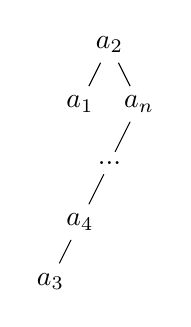
\begin{tikzpicture}[scale=0.5]
\node{$a_2$}
child{node{$a_{1}$}}
child{
	node{$a_{n}$} 
	child{
		node {...}
		child{
			node{$a_4$}
			child{
				node{$a_3$}
			}
			child[missing]
		}
		child[missing]
	} 
	child[missing] 
};
\end{tikzpicture}

In general, sequence of single rotations for $a_1, a_2, ... a_{n/2}$ takes at least $n/2$ work. Specifically, $a_1, a_2, ... a_{n/2}$ takes $n, n-1, ..., n/2$ work. In the structure above, every time a single rotation splay occurs, the subtree with $a_n$ as root doesn't change the linked list like structure, only reduces its end node's depth by 1. Splaying that end node to the top takes 1 less work than the previously splayed end node. (It the total number of nodes is odd, it will be $\lfloor n/2\rfloor$.)

\paragraph{(b)} The zig-zig operation will give the following 

\begin{tikzpicture}[scale=0.6]
\node{$a_1$}
child[missing]
child{
	node{$a_{n-1}$} 
	child{
		node {$a_{n-3}$}
		child{
			node{...}
			child{
				node{$a_4$}
				child{
					node{$a_2$}
					child[missing]
					child{node{$a_3$}}
				}
				child{node{$a_5$}}
			}
			child[missing]
		}
		child{node{$a_{n-2}$}}
	} 
	child{node{$a_{n}$}}
};
\end{tikzpicture}

This tree is better in the sense that the `overall' depth of the tree is shallower and more nodes are brought upper to the root. Notice that in (a) only node $a_1$ becomes depth 0 root and every one else increases the depth by 1 and the whole tree is essentially `equally worse' as before.

\pagebreak

\paragraph{(c)} 
First (1) we show that each node can be sinked to leaf node via a sequence of splay operations. Then (2) we show by induction that any desired shape of tree can be constructed.
\subparagraph{(1)}For sinking a node $A$ to the leaf node, consider first $A$ being a left child of some node $x$, as \begin{tikzpicture}[scale=0.5]
\node{x}
child{
	node{A} 
	child{node {y}} 
	child{node {z}} 
}
child[missing];
\end{tikzpicture}. Now considering the following two operation, (1) splay $y$'s left child, (2) splay $A$'s right child. Notice that these two operation monotonically reduces the size of $A$'s subtree. This can be seen by the following: (1) splaying $w$ of 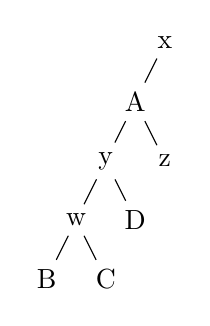
\begin{tikzpicture}[scale=0.5]
\node{x}
child{
	node{A} 
	child{
		node {y}
		child{
			node {w}
			child{node{B}}
			child{node{C}}
			}
		child{node {D}}
		} 
	child{node {z}} 
}
child[missing];
\end{tikzpicture} is 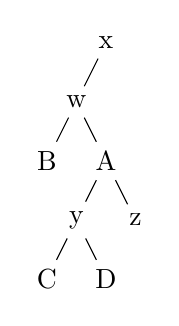
\begin{tikzpicture}[scale=0.5]
\node{x}
child{
	node{w} 
	child{node {B}} 
	child{
		node {A}
		child{
			node{y}
			child{node{C}}
			child{node{D}}
		}
		child{node{z}}
		} 
}
child[missing];
\end{tikzpicture}, which reduces the size of $A$'s subtree, (2) splaying $z$ of 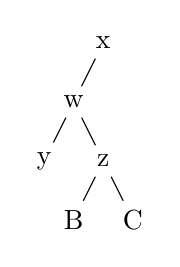
\begin{tikzpicture}[scale=0.5]
\node{x}
child{
	node{w} 
	child{node {y}} 
	child{
		node {z}
		child{node{B}}
		child{node{C}}
	} 
}
child[missing];
\end{tikzpicture} is 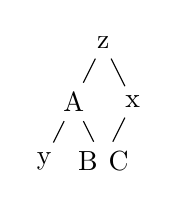
\begin{tikzpicture}[scale=0.5]
\node{z}
child{
	node{A} 
	child{node {y}} 
	child{node{B\;\;\;\;}}
}
child{node{x}
	child{node{\;\;\;\;C}}
	child[missing]};
\end{tikzpicture}, which also reduces A's subtree. Repeats either of these operation until \begin{tikzpicture}[scale=0.5]
\node{x}
child{
	node{A} 
	child{node {y}
		child[missing]
		child{node{B}}} 
	child[missing] 
}
child[missing];
\end{tikzpicture}, where $A$'s right child is missing and $y$'s left child is missing. In this case, if $y$'s right child is also empty, then we splay $y$ will make $A$ a leaf, otherwise, we use similar argument to clean up $B$'s child, then splay $B$ up, which will also make $A$ a leaf (need to clean up the children first).

(For special case $n = 1, 2, 3$, we can make a node a leaf by at most two splays of other nodes.) 

\subparagraph{(2)} 
We use mathematical induction to show this, given that in (1) we can bring any node to the leaf. First, in the trivial case $n=1$ and one splay transformation case $n=2$ we know any desired shape can be reached. Then, assuming we can reach any shape for $n$. For the case of $n+1$, we pick any node $x$ in the target shape and first sink this node to the leaf in the original tree. Then we `ignore' this leaf node in the original tree and target tree (seeing it as part of its parent node) and then do the transform as in the $n$ node case. Because node $x$ is sitting in the leaf all the time, any splay operation will not bring it up and it will just stay as a leaf. Then after the transformation it will \emph{automatically} be sitting in the right place. By mathematical induction, we reach the conclusion.

\pagebreak

\section*{Problem 4}
First we implement Access and Insert using splay trees. Then we will include reverse operation, which also modifies the implementation of access and insert but the operation amortized time is preserved. 
\subparagraph{Access and Insert} The order of the list is maintained by the tree property. When doing access element, we use find/splay operation in splay tree. The operation amortized time is $O(log\:n)$ given by splay tree find/splay. Similarly the insert operation is performed via splay tree insert, which also has am amortized time $O(log\:n)$.
\subparagraph{Reverse} For supporting Reverse, each node we add in an additional bit `reverse'. If this bit is turning on, traversing the subtree of this node will flip the left/right child, meaning that we treat left child as if it is the right child and vice versa. While traversing the tree, multiple reverse-on node may be visited, the left-right flip happens every time such reverse happens. Notice that this operation's actual cost is $O(1)$.

In the special case where $[i, j]$ is a whole subtree. Reverse(i, j) will flip the `reverse' bit in the root of the subtree. In general cases, where different parts of the trees constitute the interval, we first pre-process the tree by splaying the parts that is outside the interval to make subtrees containing only element in the interval, as in Figure \ref{fig:4-1}. Then we carry out an extended reverse operation in Figure \ref{fig:4-2}. 

\begin{figure}
	\centering
	\includegraphics[width=0.8\textwidth]{4-1.jpg}
	\caption{Preprocessing the tree by splaying the parts that is outside the interval, in order to make subtrees containing only element in the interval.} \label{fig:4-1}
\end{figure}

\emph{(Actually the \textbf{split} and \textbf{join} operation can make the following answer a lot easier. Different tree shards of the interval can be first split, cut on $i$ and $j$. Then flip the reverse bit. Then splay the nearest point to the interval (in $b$ and $d$ in Figure \ref{fig:4-2}) and then join the trees. Didn't realize this before the class.).}

In Figure \ref{fig:4-1}, shaded tree denotes nodes inside the interval. This configuration is the most `disjoint' one for the interval (notice $a$ and $b$ is single node) because of the tree property. Then we splay the root of subtree that contains nodes outside the interval. Because no more `disjoint' tree can be formed, after 2 splay operations we reach the desired state shown in Figure \ref{fig:4-1}. The splay operations take $O(log\:n)$ time. 

\begin{figure}
	\centering
	\includegraphics[width=1\textwidth]{4-2.jpg}
	\caption{Reverse operation in the general case.} \label{fig:4-2}
\end{figure}

The reverse operation applied on the desired shape in Figure \ref{fig:4-1} is shown in Figure \ref{fig:4-2}. First, flip the reverse bit on the root of $x, y, z$ and $a$ and $c$. Then flip the connection to parent node for $a$ and $c$, and for root of $y$ and $z$. While walking down the tree, $x$ is reversed, so finding larger thing is walking to the left, which results in $c$ at the end (matched with the line drawn below), which is larger than every node in $x$. Hitting reverse bit again in $c$ means left right treatment flips now, thus $d$ and $f$ is in the right order. Similar argument applies to the other direction. 

The operation of flipping reverse bit and redirect link of node is $O(1)$. Walking down the path and finding the right node takes $O(log \:n)$. Therefore the cost for this operation is $O(log\:n)$.

This reverse operation changes the standard splay operation as well. In the rotation, if a node's parent has reverse bit on, then that node and its parent flip their reverse bit in the rotation. If a node has a reverse bit on and its parent has reverse bit off, then this node turns off its reverse bit and relink its left and right child and flip their reverse bit. Other cases follow traditional splay operation. 

For illustration, denote $\bar{a}$ as the reverse bit of $a$ turning on, then in splay operation, 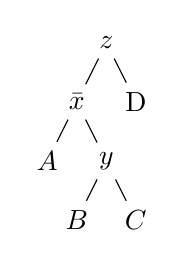
\begin{tikzpicture}[scale=0.5]
\node{$z$}
child{
	node{$\bar{x}$} 
	child{node {$A$}} 
	child{
		node {$y$}
		child{node {$B$}} 
		child{node {$C$}} 
		} 
}
child{node {D}};
\end{tikzpicture}, will become 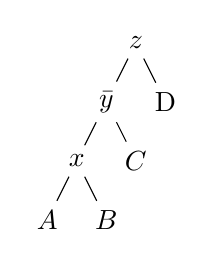
\begin{tikzpicture}[scale=0.5]
\node{$z$}
child{
	node{$\bar{y}$} 
	child{
		node {$x$}
		child{node {$A$}} 
		child{node {$B$}} 
		} 
	child{node {$C$}} 
}
child{node {D}};
\end{tikzpicture}, and then relinking and flip child nodes' reverse bit 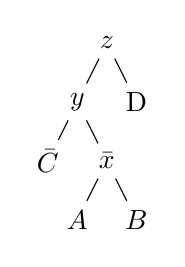
\begin{tikzpicture}[scale=0.5]
\node{$z$}
child{
	node{$y$} 
	child{node {$\bar{C}$}} 
	child{
		node {$\bar{x}$}
		child{node {$A$}} 
		child{node {$B$}} 
	} 
}
child{node {D}};
\end{tikzpicture} and then carry out the normal rotation to reach 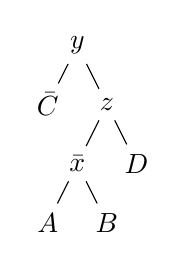
\begin{tikzpicture}[scale=0.5]
\node{$y$}
child{node {$\bar{C}$}}
child{
	node{$z$} 
	child{
		node {$\bar{x}$}
		child{node {$A$}} 
		child{node {$B$}} 
	}
	child{node {$D$}} 
};
\end{tikzpicture}. The correctness is followed by the notion of reverse bit and tree property. In each rotation, the cost is still $O(1)$ as for flipping bit and changing child node connection. Therefore the amortized cost for splay still holds.

\section*{Problem 5}
\paragraph{(a)} The intuition is that the more `balanced' it is the faster walking down the tree it is. The largest amount of balance triple can be hit by always following a path that has slightly less than $9/10$ of top of triple's descendants. Walking down such search path, the depth reduces by $9/10 -\epsilon$, where $\epsilon$ is the min of the slight decrement from $9/10$ along the search path. Then the number of triple is bounded by $log_{1/(9/10 - \epsilon)}\: n$, which is $O(log\:n)$.
\paragraph{(b)} Biased means most mass is in $x$'s subtree. In zig-zig case, 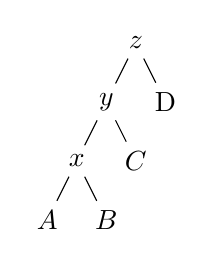
\begin{tikzpicture}[scale=0.5]
\node{$z$}
child{
	node{$y$} 
	child{
		node {$x$}
		child{node {$A$}} 
		child{node {$B$}} 
	} 
	child{node {$C$}} 
}
child{node {D}};
\end{tikzpicture} will be converted into 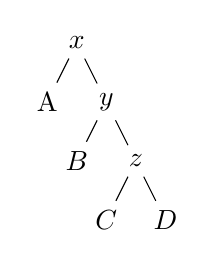
\begin{tikzpicture}[scale=0.5]
\node{$x$}
child{node {A}}
child{
	node{$y$} 
	child{node {$B$}}
	child{
		node {$z$}
		child{node {$C$}} 
		child{node {$D$}} 
	}  
};
\end{tikzpicture}. Either $A$ or $B$ (or collectively both) has the dominant mass, then $z$ significantly reduces its rank by at least $8/10 \: log \: n$ while $x$ only add at most $1/10\: log\:n$.

Similarly, in zig-zag case, 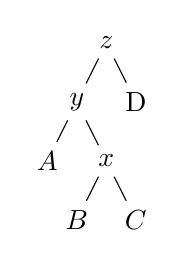
\begin{tikzpicture}[scale=0.5]
\node{$z$}
child{
	node{$y$} 
	child{node {$A$}} 
	child{
		node {$x$}
		child{node {$B$}} 
		child{node {$C$}} 
	} 
}
child{node {D}};
\end{tikzpicture} will be converted to 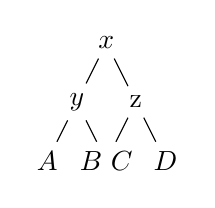
\begin{tikzpicture}[scale=0.5]
\node{$x$}
child{
	node{$y$} 
	child{node {$A$}} 
	child{node {$B$\;\;\;\;}}
}
child{
	node {z}
	child{node {\;\;\;\;$C$}} 
	child{node {$D$}}
	};
\end{tikzpicture} where most of the mass is in $B$ and $C$. If $B$ has dominant mass, then $z$ reduces its potential significantly by $9/10 \: log\: - 1 - \epsilon$ where $\epsilon$ is due to $C$, and vice versa when $C$ dominants. If $B$ and $C$ split the mass, then both $y$ and $z$ will reduce potential by at least $4/10 \: log\: n$. x only increases its potential by $2/10 \: log\: n$. 

\pagebreak

\paragraph{(c)} From the tree plot in (b), notice that only $x, y, z$ can change rank. In zig-zig case, the potential difference is 
\begin{align*}
&\;\;\;\;\; r'(z) + r'(y) + r'(x) - r(x) - r(y) - r(z)\\
&= r'(z) +r'(y) - r(x) - r(y) \;\; \big(\text{from tree structure, } r(z) = r'(x)\big)\\
&\leq 2\big( r(z) -  r(x)\big) \;\; \big(\text{because } r'(z) < r'(y) < r(z), \; r(y) > r(x)\big)\\
\end{align*}
Likewise, from the plot in (b), in zig-zag case the potential difference is 
\begin{align*}
&\;\;\;\;\; r'(z) + r'(y) + r'(x) - r(x) - r(y) - r(z)\\
&= r'(z) +r'(y) - r(x) - r(y) \;\; \big(\text{from tree structure, } r(z) = r'(x)\big)\\
&\leq 2\big( r(z) -  r(x)\big) \;\; \big(\text{because } r'(z) < r'(y) < r(z), \; r(y) > r(x)\big)\\
\end{align*}

(Notice that $r(z)$ is at the top and has highest rank, $r(x)$ is at the lowest of the triple and has the lowest rank, in both graphs. A sanity check.)

\paragraph{(d)} From (b) we see significant potential being fell out the system if the triple is biased, that means the biased case can be put aside in the amortized cost analysis. The potential increase in balanced case is bounded by $2\big( r(z) -  r(x)\big)$, which bounded by $O(log\:n)$, as the mass outside $x$ is bounded by $1/10$ of the total. Since there is $O(log\:n)$ balanced rotation in (a), where each takes $O(1)$, By $\text{cost}_{amortized} = \text{cost}_{real} + \Delta{\Phi}$ and by (c) the potential difference telescopes, we know amortized cost is bounded by $O(log\:n)$. 

\end{document}
